\title{
	CSCI547 Machine Learning\\
	Homework 2\\
}
\author{
	Zachary Falkner\\
	Department of Computer Science\\
	University of Montana\\
}
\date{\today}
\documentclass[12pt]{article}

\usepackage{enumitem, listings, graphicx, xcolor, amsmath}

\lstset{language=Python,
	keywordstyle=\color{blue},
	basicstyle=\scriptsize\ttfamily,
	commentstyle=\ttfamily\itshape\color{gray},
	stringstyle=\ttfamily,
	showstringspaces=false,
	breaklines=true,
	frameround=ffff,
	frame=single,
	rulecolor=\color{black}
}

\begin{document}
	\maketitle
	
	\begin{flushleft}
		\section{Logistic Regression}
		
		\subsection*{1A}
		\begin{lstlisting}
import numpy as np 
import pandas as pd


# The sigmoid function
def _sigmoid(w,X):
	z = np.dot(X,w)
	return 1./(1+np.exp(-z))


# The objective function
def _J_fun(w,X,y):
	return -sum(y*np.log(_sigmoid(w,X)) + (1-y)*np.log(1-_sigmoid(w,X)))


# The gradient of the objective function
def _gradient_fun(w,X,y):
	return np.dot(_sigmoid(w,X)-y,X)


class LogisticRegression:
	def __init__(self, eta=None, epochs=10000, w=None):
		self.eta= eta
		self.epochs = epochs
		self.w = w
		self.cost_over_epochs = []
	
	
	def fit(self, x, y):
		N = len(y)
		
		for i in range(self.epochs):
		grad_w = _gradient_fun(self.w,x,y)    # Compute the gradient of the objective function
		self.w -= np.dot(self.eta,grad_w)
		self.cost_over_epochs.append(_J_fun(self.w,x,y))
		
		classification_error = sum((_sigmoid(self.w,x)>0.5)==y)/N
		return classification_error
	
	
	def score(self, x, y):
		N = len(y)
		
		classification_error = sum((_sigmoid(self.w,x)>0.5)==y)/N
		return classification_error


		\end{lstlisting}
		\begin{lstlisting}
import numpy as np 
import pandas as pd

from logistic_regression import LogisticRegression


if __name__ == '__main__':
	DATAFILE = 'lobster_survive.dat'
	df = pd.read_csv(DATAFILE,header=0, sep=r"\s{2,}")
	x = df.iloc[:, 0].as_matrix().astype(float)
	y = df.iloc[:, 1].as_matrix().astype(float)
	x = np.vander(x,2,increasing=True)
	
	
	#learning rate, tensor
	eta = np.array([[0.000001,0],[0,0.000000001]])
	
	#number of iterations
	epochs = 200000
	
	#weights
	w = np.array([-1.,0.5])
	
	lr = LogisticRegression(eta=eta, epochs=epochs, w=w)
	error = lr.fit(x, y)
	print("classification error: {}".format(error))



		\end{lstlisting}
		
		classification error: 0.710691823899371
		
		\subsection*{1B}
		\begin{lstlisting}
import numpy as np 
import pandas as pd
import matplotlib.pyplot as plt
from scipy.stats import zscore

from logistic_regression import LogisticRegression


if __name__ == '__main__':
	TRAINFILE = 'titanic_train.csv'
	TESTFILE = 'titanic_test.csv'
	train_df = pd.read_csv(TRAINFILE,header=0)
	test_df = pd.read_csv(TESTFILE,header=0)
	
	x_data = train_df.iloc[:, 2:]
	
	# drop useless columns
	x_data.drop(['Cabin', 'Ticket', 'Name'], axis=1, inplace=True)
	
	# one hot sex and embarked
	x_data = pd.get_dummies(x_data, columns=['Sex', 'Embarked'])
	
	# fill missing age data with mean....
	x_data['Age'] = x_data['Age'].fillna(x_data['Age'].mean())
	
	# normalize with zscores
	numeric_cols = ['Parch', 'SibSp', 'Age', 'Fare']
	x_data[numeric_cols] = x_data[numeric_cols].apply(zscore)
	
	x = x_data.as_matrix().astype(float)
	y = train_df.iloc[:, 1].as_matrix().astype(float)
	
	
	x_data_test = test_df.iloc[:, 2:]
	
	# drop useless columns
	x_data_test.drop(['Cabin', 'Ticket', 'Name'], axis=1, inplace=True)
	
	# one hot sex and embarked
	x_data_test = pd.get_dummies(x_data_test, columns=['Sex', 'Embarked'])
	
	# fill missing age data with mean....
	x_data_test['Age'] = x_data_test['Age'].fillna(x_data_test['Age'].mean())
	
	# normalize with zscores
	x_data_test[numeric_cols] = x_data_test[numeric_cols].apply(zscore)
	
	x_test = x_data_test.as_matrix().astype(float)
	y_test = test_df.iloc[:, 1].as_matrix().astype(float)
	
	#learning rate, tensor
	eta = np.eye(10) * np.array([0.000001] * 10)
	
	#number of iterations
	epochs = 200000
	
	#weights
	w = np.array([-1.,0.5,0.5,0.5,0.5,0.5,0.5,0.5,0.5,0.5])
	
	lr = LogisticRegression(eta=eta, epochs=epochs, w=w)
	
	error = lr.fit(x, y)
	print("training error: {}".format(error))
	
	test_error = lr.score(x_test, y_test)
	print("test error: {}".format(test_error))
	
	iterations = len(lr.cost_over_epochs)
	print("training iterations: {}".format(iterations))
	
	plt.plot(lr.cost_over_epochs, 'k')
	plt.xlabel('training iterations N')
	plt.ylabel('cost')
	plt.show()

		\end{lstlisting}
		
		training error: 0.7962962962962963\\
		test error: 0.8047138047138047\\
		training iterations: 100000\\
		
		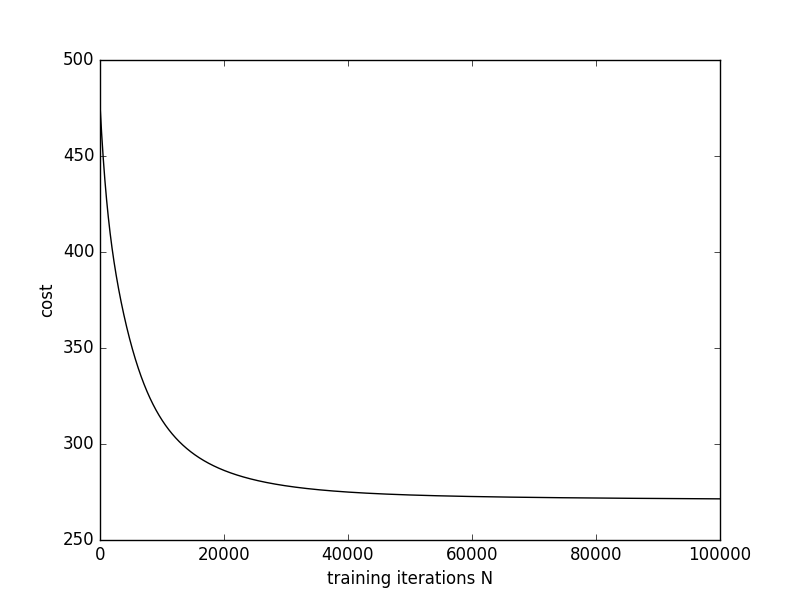
\includegraphics[scale=0.5]{HW2_1B.png}
		\label{fig:graph 1B}
		
		\subsection*{1C*}
		
		\begin{lstlisting}
import numpy as np 
import pandas as pd


# The sigmoid function
def _sigmoid(w,X):
	z = np.dot(X,w)
	return 1./(1+np.exp(-z))


# The objective function
def _J_fun(w,X,y):
	return -sum(y*np.log(_sigmoid(w,X)) + (1-y)*np.log(1-_sigmoid(w,X)))


# The gradient of the objective function
def _gradient_fun(w,X,y):
	return np.dot(_sigmoid(w,X)-y,X)


class LogisticRegression:
	def __init__(self, eta=None, epochs=10000, w=None, enable_early_stop=False, early_stop_tolerance=10):
		self.eta= eta
		self.epochs = epochs
		self.w = w
		self.cost_over_epochs = []
		self.gradiant_over_epochs = []
		
		self.enable_early_stop = enable_early_stop
		self.early_stop_tolerance = early_stop_tolerance
	
	
	def fit(self, x, y):
		N = len(y)
		
		for i in range(self.epochs):
			grad_w = _gradient_fun(self.w,x,y)    # Compute the gradient of the objective function
			self.w -= np.dot(self.eta,grad_w)
			self.cost_over_epochs.append(_J_fun(self.w,x,y))
			self.gradiant_over_epochs.append(grad_w)
			
			if(self.shouldTerminateEarly()):
				break;
	
		classification_error = sum((_sigmoid(self.w,x)>0.5)==y)/N
		return classification_error
	
	
	def score(self, x, y):
		N = len(y)
		
		classification_error = sum((_sigmoid(self.w,x)>0.5)==y)/N
		return classification_error
	
	def shouldTerminateEarly(self):
		if(self.enable_early_stop == True):
			grads = self.gradiant_over_epochs[-1]
			return (all(g < self.early_stop_tolerance for g in grads)
			and all(g > -1 * self.early_stop_tolerance for g in grads) )
			return False

		\end{lstlisting}
		
		\begin{lstlisting}
import numpy as np 
import pandas as pd
import matplotlib.pyplot as plt
from scipy.stats import zscore

from logistic_regression import LogisticRegression


if __name__ == '__main__':
TRAINFILE = 'titanic_train.csv'
TESTFILE = 'titanic_test.csv'
train_df = pd.read_csv(TRAINFILE,header=0)
test_df = pd.read_csv(TESTFILE,header=0)

x_data = train_df.iloc[:, 2:]

# drop useless columns
x_data.drop(['Cabin', 'Ticket', 'Name'], axis=1, inplace=True)

# one hot sex and embarked
x_data = pd.get_dummies(x_data, columns=['Sex', 'Embarked'])

# fill missing age data with mean....
x_data['Age'] = x_data['Age'].fillna(x_data['Age'].mean())

# normalize with zscores
numeric_cols = ['Parch', 'SibSp', 'Age', 'Fare']
x_data[numeric_cols] = x_data[numeric_cols].apply(zscore)

x = x_data.as_matrix().astype(float)
y = train_df.iloc[:, 1].as_matrix().astype(float)


x_data_test = test_df.iloc[:, 2:]

# drop useless columns
x_data_test.drop(['Cabin', 'Ticket', 'Name'], axis=1, inplace=True)

# one hot sex and embarked
x_data_test = pd.get_dummies(x_data_test, columns=['Sex', 'Embarked'])

# fill missing age data with mean....
x_data_test['Age'] = x_data_test['Age'].fillna(x_data_test['Age'].mean())

# normalize with zscores
x_data_test[numeric_cols] = x_data_test[numeric_cols].apply(zscore)

x_test = x_data_test.as_matrix().astype(float)
y_test = test_df.iloc[:, 1].as_matrix().astype(float)

#learning rate, tensor
eta = np.eye(10) * np.array([0.000001] * 10)

#number of iterations
epochs = 100000

#weights
w = np.array([-1.,0.5,0.5,0.5,0.5,0.5,0.5,0.5,0.5,0.5])

lr = LogisticRegression(eta=eta, epochs=epochs, w=w, enable_early_stop=True, early_stop_tolerance=10)

error = lr.fit(x, y)
print("training error: {}".format(error))

test_error = lr.score(x_test, y_test)
print("test error: {}".format(test_error))

iterations = len(lr.cost_over_epochs)
print("training iterations: {}".format(iterations))

plt.plot(lr.cost_over_epochs, 'k')
plt.plot(lr.gradiant_over_epochs, 'r')
plt.xlabel('training iterations N')
plt.ylabel('gradiants, cost')
plt.show()

		\end{lstlisting}
		
		
		training error: 0.7962962962962963\\
		test error: 0.8080808080808081\\
		training iterations: 45137\\
		
		for this i plotted cost and gradients over iterations and noticed that when the gradients all converge towards 0 the cost is converging. seems sound, got similar results with less than 1/4 the iterations.\\
		
		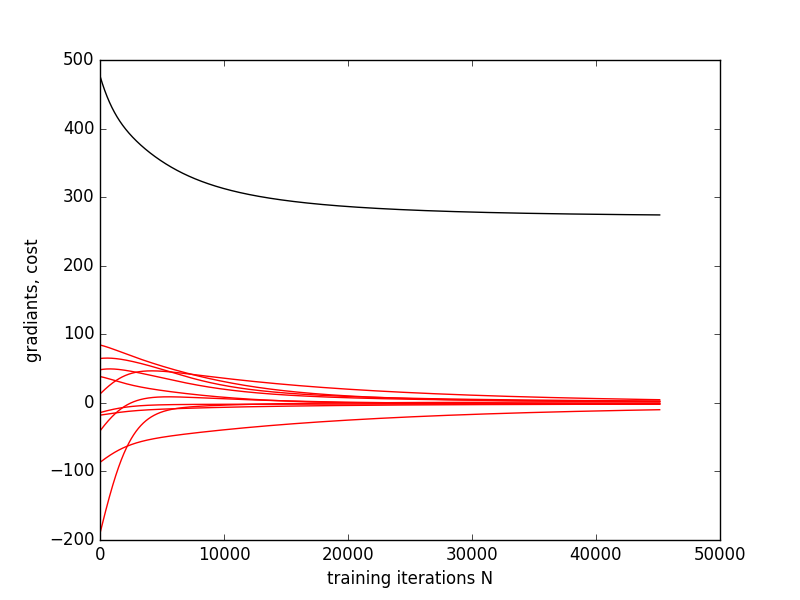
\includegraphics[scale=0.5]{HW2_1C.png}
		\label{fig:graph 1C}

		
		\section{Neural Networks}
		
		\subsection*{2A}
		Ok, Done!\\
		
		\subsection*{2B}
		\begin{lstlisting}
from __future__ import division,print_function

import numpy as np

class Network(object):
"""
Neural network for softmax regression problems
"""

def __init__(self,layer_number_of_nodes,layer_activation_functions,layer_has_bias,layer_weight_means_and_stds=None):
	self.layer_number_of_nodes = layer_number_of_nodes           # Of nodes in each layer
	self.layer_activation_functions = [None]
	# Add an identity activation function here!
	for act in layer_activation_functions:
		if act=='softmax':
			self.layer_activation_functions.append(self._softmax) 
		if act=='sigmoid':
			self.layer_activation_functions.append(self._sigmoid) 
		if act=='leaky_relu':
			self.layer_activation_functions.append(self._leaky_relu) 
		if act=='gaussian':
			self.layer_activation_functions.append(self._gaussian) 
		if act=='identity':
			self.layer_activation_functions.append(self._identity)
	
	self.layer_has_bias = layer_has_bias                         # Whether to add a bias node to each layer
	self.L = len(self.layer_number_of_nodes)                     # Number of layers
	
	self.weights = [np.array([])]
	
	# Create arrays to hold the weights, which are N_l(+1) by N_(l+1)
	for i in range(self.L-1):
		# if we have a normal distribution and standard deviation, then generate random weights from that distribution,
		if layer_weight_means_and_stds is not None:
			w = layer_weight_means_and_stds[i][1]*np.random.randn(self.layer_number_of_nodes[i] + self.layer_has_bias[i],self.layer_number_of_nodes[i+1]) + layer_weight_means_and_stds[i][0] 
		# Otherwise just initialize the weights to zero
		else:
			w = np.zeros((self.layer_number_of_nodes[i] + self.layer_has_bias[i],self.layer_number_of_nodes[i+1]))
		self.weights.append(w)

def feed_forward(self,feature):
	# evaluate the neural network for a vector-valued input
	m = feature.shape[0]
	
	# Append a column of ones to the input if a bias is desired
	if self.layer_has_bias[0]:
		z = np.column_stack((np.ones((m)),feature))
	else:
		z = feature
	
	# Initialize lists to hold the node inputs and outputs, treating the input values as the output of the first node
	self.a_vals = [None]
	self.z_vals = [z]
	
	# Loop over the remaining layers
	for l in range(1,self.L):
		# Take the linear combination of the previous layers outputs (z^(l-1)) and weights (w^(l)) to form a^(l)
		a = np.dot(self.z_vals[l-1],self.weights[l])
		# Run a through the activation function to form z^(l)
		z = self.layer_activation_functions[l](a) 
		# If a bias is desired, append a column of ones to z
		if self.layer_has_bias[l]:         
		z = np.column_stack((np.ones((m)),z))
		# Store these values (for computing the gradient later)
		self.a_vals.append(a) 
		self.z_vals.append(z)
	return z

def _J_fun(self,feature,label):
	# Add your sum square error evaluation here!
	if self.layer_activation_functions[-1]==self._identity:
		cost_function_data = np.sum(np.sum((1/2) * np.power(label - self.feed_forward(feature), 2), axis=1), axis=0)
	if self.layer_activation_functions[-1]==self._softmax:
		# Model objective function -- Cross-entropy 
		cost_function_data = -np.sum(np.sum(label*np.log(self.feed_forward(feature)),axis=1),axis=0)
	else:
		print('Only softmax supported for final layer')            
	
	# Add regularization here!
	# TODO
	cost_function_reg = 0
	return cost_function_data + cost_function_reg

def _gradient_fun(self,feature,label):
	# Compute the gradient via backpropagation
	m = feature.shape[0]
	
	# Initialize gradient arrays (same shape as the weights)
	grads = [np.zeros_like(w) for w in self.weights]
	
	# Compute dJ/da (aka the delta term) for the final layer.  This often involves 
	# Some algebraic simplification when cost function is selected judiciously, so
	# this is coded by hand here.
	
	l = self.L-1 #last layer
	
	z = self.z_vals[l]              # Current layer out
	z_previous = self.z_vals[l-1]   # Last layer out
	a = self.a_vals[l]              # Current layer in
	w = self.weights[l]             # Last layer weights
	activation = self.layer_activation_functions[l]     #Current layer activation
	if activation==self._softmax or activation==self._identity:
		delta_l = (z - label)                       # Current layer error
	# Add gradient of SSE here!
	else:
		print('Only softmax and identity supported for final layer') 
	
	grads[l] = np.dot(z_previous.T,delta_l)    # gradient due to data misfit
	
	# Add gradient of regularization here!
	model_norm_gradient = 0
	grads[l] += model_norm_gradient                    # add gradient due to regularization
	
	# Loop over the remaining layers
	for l in range(self.L-2,0,-1):
	
		z_previous = self.z_vals[l-1]                    # last layer output
		a = self.a_vals[l]                                # Current layer input
		
		w_next = self.weights[l+1][1:] # weights from the next layer, excluding bias weights
		activation = self.layer_activation_functions[l]  # Current layer activation
		
		delta_l = np.dot(delta_l,w_next.T)*activation(a,dx=1)  # Current layer error
		grads[l] = np.dot(z_previous.T,delta_l)  # Gradient due to data misfit
		
		# Add gradient of regularization here!
		model_norm_gradient = 0
		grads[l] += model_norm_gradient             # add gradient due to regularization
	
	return grads

@staticmethod
def _softmax(X,dx=0):
	if dx==0:
		return np.exp(X)/np.repeat(np.sum(np.exp(X),axis=1,keepdims=True),X.shape[1],axis=1)
@staticmethod
def _sigmoid(X,dx=0):
	if dx==0:
		return 1./(1+np.exp(-X))
	if dx==1:
	s = 1./(1+np.exp(-X))
		return s*(1-s)

@staticmethod
def _leaky_relu(X,dx=0):
	if dx==0:
		return (X>0)*X + 0.01*(X<=0)*X
	if dx==1:
		return (X>0) + 0.01*(X<=0)

@staticmethod
def _gaussian(X,dx=0):
	if dx==0:
		return np.exp(-X**2)
	if dx==1:
		return -2*X*np.exp(-X**2)

# Add @staticmethod for identity here
@staticmethod
def _identity(X,dx=0):
	if dx == 0:
		return X 
	return np.onelike(X)

		\end{lstlisting}
		
		\begin{lstlisting}
import numpy as np
import matplotlib.pyplot as plt

from neural_network import Network


if __name__ == '__main__':
	n = 1
	m = 100
	N = 1
	X = np.random.rand(m, 1)
	y = np.exp(-np.sin(np.power(X, 3) * 4 * np.pi))
	
	X_test = np.random.rand(m, 1)
	y_test = np.exp(-np.sin(np.power(X_test, 3) * 4 * np.pi))
	
	nn = Network([n,20,N],[None,'sigmoid','identity'],[True,True,False],layer_weight_means_and_stds=[(0,0.1),(0,0.1)])
	
	eta = 0.001
	
	N_iterations = 10000
	
	T = y
	
	# Perform gradient descent
	for i in range(N_iterations):
		
		# For stochastic gradient descent, take random samples of X and T
		
		# Run the features through the neural net (to compute a and z)
		y_pred = nn.feed_forward(X)
		
		# Compute the gradient
		grad_w = nn._gradient_fun(X,T) 
		
		# Update the neural network weight matrices
		for w,gw in zip(nn.weights,grad_w):
			w -= eta*gw
		
		# Print some statistics every thousandth iteration
		if i%1000==0:
			misclassified = sum(np.argmax(y_pred,axis=1)!=y.ravel())
			print ("Iteration: {0}, Objective Function Value: {1:3f}, Misclassified: {2}".format(i,nn._J_fun(X,T), misclassified))
	
	# Predict the training data and classify
	y_pred = np.argmax(nn.feed_forward(X_test),axis=1)
	print ("Test data accuracy: {0:3f}".format(1-sum(y_pred!=y_test.ravel())/float(len(y_test))))

		\end{lstlisting}
		
		\subsection*{2C}
		\begin{lstlisting}
from __future__ import division,print_function

import numpy as np

class Network(object):
"""
Neural network for softmax regression problems
"""

def __init__(self,layer_number_of_nodes,layer_activation_functions,layer_has_bias,layer_weight_means_and_stds=None, gama=0.1, regularization=None):
	self.layer_number_of_nodes = layer_number_of_nodes           # Of nodes in each layer
	self.layer_activation_functions = [None]
	# Add an identity activation function here!
	for act in layer_activation_functions:
		if act=='softmax':
			self.layer_activation_functions.append(self._softmax) 
		if act=='sigmoid':
			self.layer_activation_functions.append(self._sigmoid) 
		if act=='leaky_relu':
			self.layer_activation_functions.append(self._leaky_relu) 
		if act=='gaussian':
			self.layer_activation_functions.append(self._gaussian) 
		if act=='identity':
			self.layer_activation_functions.append(self._identity)
	
	self.layer_has_bias = layer_has_bias                         # Whether to add a bias node to each layer
	self.L = len(self.layer_number_of_nodes)                     # Number of layers
	self.gama = gama
	
	self.weights = [np.array([])]
	self.regularization = regularization
	
	# Create arrays to hold the weights, which are N_l(+1) by N_(l+1)
	for i in range(self.L-1):
		# if we have a normal distribution and standard deviation, then generate random weights from that distribution,
		if layer_weight_means_and_stds is not None:
			w = layer_weight_means_and_stds[i][1]*np.random.randn(self.layer_number_of_nodes[i] + self.layer_has_bias[i],self.layer_number_of_nodes[i+1]) + layer_weight_means_and_stds[i][0] 
		# Otherwise just initialize the weights to zero
		else:
			w = np.zeros((self.layer_number_of_nodes[i] + self.layer_has_bias[i],self.layer_number_of_nodes[i+1]))
		self.weights.append(w)

def feed_forward(self,feature):
	# evaluate the neural network for a vector-valued input
	m = feature.shape[0]

	# Append a column of ones to the input if a bias is desired
	if self.layer_has_bias[0]:
		z = np.column_stack((np.ones((m)),feature))
	else:
		z = feature
	
	# Initialize lists to hold the node inputs and outputs, treating the input values as the output of the first node
	self.a_vals = [None]
	self.z_vals = [z]
	
	# Loop over the remaining layers
	for l in range(1,self.L):
		# Take the linear combination of the previous layers outputs (z^(l-1)) and weights (w^(l)) to form a^(l)
		a = np.dot(self.z_vals[l-1],self.weights[l])
		# Run a through the activation function to form z^(l)
		z = self.layer_activation_functions[l](a) 
		# If a bias is desired, append a column of ones to z
		if self.layer_has_bias[l]:         
			z = np.column_stack((np.ones((m)),z))
		# Store these values (for computing the gradient later)
		self.a_vals.append(a) 
		self.z_vals.append(z)
	return z

def _J_fun(self,feature,label):
	# Add your sum square error evaluation here!
	if self.layer_activation_functions[-1]==self._identity:
		cost_function_data = np.sum(np.sum((1/2) * np.power(label - self.feed_forward(feature), 2), axis=1), axis=0)
	if self.layer_activation_functions[-1]==self._softmax:
		# Model objective function -- Cross-entropy 
		cost_function_data = -np.sum(np.sum(label*np.log(self.feed_forward(feature)),axis=1),axis=0)
	else:
		print('Only softmax supported for final layer')            
	
	# Add regularization here!
	# TODO
	cost_function_reg = 0
	if(self.regularization == 'L1'):
		for w in self.weights:
			cost_function_reg = self.gama * np.sum(np.abs(w))
	if(self.regularization == 'L2'):
		for w in self.weights:
			cost_function_reg = self.gama * np.sum(np.power(w, 2))
	
	return cost_function_data + cost_function_reg

def _gradient_fun(self,feature,label):
	# Compute the gradient via backpropagation
	m = feature.shape[0]
	
	# Initialize gradient arrays (same shape as the weights)
	grads = [np.zeros_like(w) for w in self.weights]
	
	# Compute dJ/da (aka the delta term) for the final layer.  This often involves 
	# Some algebraic simplification when cost function is selected judiciously, so
	# this is coded by hand here.
	
	l = self.L-1 #last layer

	z = self.z_vals[l]              # Current layer out
	z_previous = self.z_vals[l-1]   # Last layer out
	a = self.a_vals[l]              # Current layer in
	w = self.weights[l]             # Last layer weights
	activation = self.layer_activation_functions[l]     #Current layer activation
	if activation==self._softmax or activation==self._identity:
		delta_l = (z - label)                       # Current layer error
	# Add gradient of SSE here!
	else:
		print('Only softmax and identity supported for final layer') 

	grads[l] = np.dot(z_previous.T,delta_l)    # gradient due to data misfit

	# Add gradient of regularization here!
	model_norm_gradient = 0
	if(self.regularization == 'L1'):
		model_norm_gradient = self.gama * np.sign(w)
	if(self.regularization == 'L2'):
		model_norm_gradient = self.gama * w
	grads[l] += model_norm_gradient                    # add gradient due to regularization
	
	# Loop over the remaining layers
	for l in range(self.L-2,0,-1):
	
		z_previous = self.z_vals[l-1]                    # last layer output
		a = self.a_vals[l]                                # Current layer input
		
		w_next = self.weights[l+1][1:] # weights from the next layer, excluding bias weights
		activation = self.layer_activation_functions[l]  # Current layer activation
		
		delta_l = np.dot(delta_l,w_next.T)*activation(a,dx=1)  # Current layer error
		grads[l] = np.dot(z_previous.T,delta_l)  # Gradient due to data misfit
		
		# Add gradient of regularization here!
		model_norm_gradient = 0
		if(self.regularization == 'L1'):
			model_norm_gradient = self.gama * np.sign(self.weights[l])
		if(self.regularization == 'L2'):
			model_norm_gradient = self.gama * self.weights[l]
		grads[l] += model_norm_gradient             # add gradient due to regularization
	
	return grads

@staticmethod
def _softmax(X,dx=0):
	if dx==0:
		return np.exp(X)/np.repeat(np.sum(np.exp(X),axis=1,keepdims=True),X.shape[1],axis=1)
@staticmethod
def _sigmoid(X,dx=0):
	if dx==0:
		return 1./(1+np.exp(-X))
	if dx==1:
		s = 1./(1+np.exp(-X))
		return s*(1-s)

@staticmethod
def _leaky_relu(X,dx=0):
	if dx==0:
		return (X>0)*X + 0.01*(X<=0)*X
	if dx==1:
		return (X>0) + 0.01*(X<=0)

@staticmethod
def _gaussian(X,dx=0):
	if dx==0:
		return np.exp(-X**2)
	if dx==1:
		return -2*X*np.exp(-X**2)

# Add @staticmethod for identity here
@staticmethod
def _identity(X,dx=0):
	if dx == 0:
		return X 
	return np.onelike(X)

		\end{lstlisting}
		
		\subsection*{2D}
		I overextended my schedule this week and did not get to complete 2D or 2E.
		
		\subsection*{2E*}
		...
		
		\section{TensorFlow}
		
		\subsection*{3A}
		\begin{lstlisting}
import matplotlib.pyplot as plt

...

# You can acquire the values of your layer weights with
w = sess.run(W_0)
w = w.reshape(10, 28, 28)

fig, axes = plt.subplots(2, 5, subplot_kw={'xticks': [], 'yticks': []})

for ax, x in zip(axes.flat, w):
ax.imshow(x, interpolation=None, cmap='viridis')

plt.show()

		\end{lstlisting}
		
		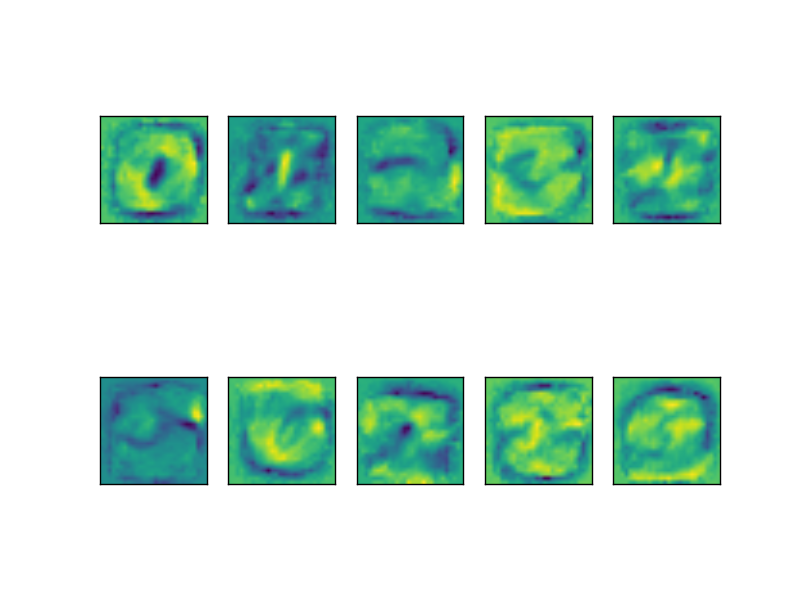
\includegraphics[scale=0.5]{HW2_3A.png}
		\label{fig:graph 3A}
		
		\subsection*{3B}
		\begin{lstlisting}
import argparse
import sys
import matplotlib.pyplot as plt

from tensorflow.examples.tutorials.mnist import input_data

import tensorflow as tf


# Tensorflow has the mnist data builtin
data_dir = '/tmp/tensorflow/mnist/input_data'

# Import data
mnist = input_data.read_data_sets(data_dir,one_hot=True)

n = 784  # Number of input features
N = 10   # Number of classes

# X is the vector of inputs (though it's just a placeholder until a tensorflow session is started)
X = tf.placeholder("float", [None, n])

# y is the vector of targets
y = tf.placeholder("float", [None, N])

# Create the model
# layer 1 weights and biases
W_0 = tf.Variable(tf.random_normal([n,N],stddev=0.01))
b_0 = tf.Variable(tf.random_normal([N],stddev=0.01))

# Create neural network
def multilayer_perceptron(x):
	out_layer = tf.add(tf.matmul(x,W_0),b_0)
	hidden_layer = tf.layers.dense(inputs=out_layer, units=300, activation=tf.nn.sigmoid)
	logits = tf.layers.dense(inputs=hidden_layer, units=10)
	return logits

# define prediction object
y_pred = multilayer_perceptron(X)

# Define loss function (combined softmax and cross-entropy output) 
loss_op = tf.reduce_sum(tf.nn.softmax_cross_entropy_with_logits(logits=y_pred, labels=y))

# Specify learning rate
learning_rate = 0.001

# Define optimization step
optimizer = tf.train.AdamOptimizer(learning_rate=learning_rate)

# The optimization procedure (minimizing the softmax cross_entropy)
train_op = optimizer.minimize(loss_op)

# Initialize all the variables
# (tensorflow doesn't compute variable values unless run by as session)
sess = tf.InteractiveSession()
init  = tf.global_variables_initializer().run()

# Train
N_iterations = 200000
sample_size = 10

for i in range(N_iterations):
	
	# Pull a sample from the training set
	batch_xs, batch_ys = mnist.train.next_batch(sample_size)
	
	# Run tensor flow objects: train_op updates the weights, loss_op compute the cost function
	_,c = sess.run([train_op,loss_op], feed_dict={X: batch_xs, y: batch_ys})
	
	# Print statistics every 1000 steps
	if i%1000==0:
		# Test trained model
		pred = tf.nn.softmax(y_pred)
		correct_prediction = tf.equal(tf.argmax(pred, 1), tf.argmax(y,1))
		accuracy = tf.reduce_mean(tf.cast(correct_prediction, tf.float32))
		print("Accuracy:", accuracy.eval({X: mnist.test.images, y: mnist.test.labels}),c)

# You can acquire the values of your layer weights with
# w = sess.run(W_0)
# w = w.reshape(10, 28, 28)

# fig, axes = plt.subplots(2, 5, subplot_kw={'xticks': [], 'yticks': []})

# for ax, x in zip(axes.flat, w):
#     ax.imshow(x, interpolation=None, cmap='viridis')

# plt.show()

		\end{lstlisting}
		
	\end{flushleft}
\end{document}